\documentclass[10pt]{article}
\usepackage[margin=0.85in]{geometry}
\usepackage{booktabs}
\usepackage{microtype}
\usepackage{parskip}
\usepackage{titlesec}
\usepackage{hyperref}
\usepackage{graphicx}
\usepackage{caption}

\titleformat{\section}{\normalfont\bfseries\large}{\thesection}{0.6em}{}
\titlespacing*{\section}{0pt}{0.8em}{0.2em}
\captionsetup{font=small,labelfont=bf,skip=4pt}

\title{\vspace{-2.5em}\textbf{Language models decide \emph{what kind} of fact before they decide \emph{which} fact}\vspace{-0.5em}}
\author{}
\date{}

\begin{document}
\maketitle
\vspace{-3em}

\section*{The question, in one line}

\emph{The capital of France is \_\_\_} which a capable language model should say \emph{Paris}. But when the model decides on \emph{Paris}, has it already settled on the relation \emph{capital-of} first, or do both pieces click into place at the same time? I tested four models and found a robust ordering at the final token: relation information becomes generation-controlling first, entity-specific answer information second, by a wide margin.

\section*{The setup}

Two terms I'll use throughout. \textbf{Relation} = the kind of fact being looked up (\emph{capital-of}, \emph{past-tense-of}, \emph{opposite-of}). \textbf{Entity} = the specific input the relation applies to (\emph{France}, \emph{walk}, \emph{hot}). The question I'm asking is: at the final token where the answer is generated, when does relation information become \emph{generation-controlling}, and when does entity information?

The core tool is activation patching at the final-token position: at a chosen layer $\ell$, I take a donor prompt's hidden state at its final token, paste it into the recipient's final token, and check whether the recipient's first generated answer flips toward the donor-compatible answer. Sweep $\ell$ across the network and you get a transfer curve. \textbf{Onset} = the first layer where transfer crosses 0.4 for two consecutive tested layers.

Two key conditions: \textbf{relation transfer} (same entity, different relation --- recipient \emph{capital(France)} + donor \emph{language(France)}, success = \emph{French}) tests whether the final token is controlled by relation-type information; \textbf{entity transfer} (same relation, different entity --- recipient \emph{capital(France)} + donor \emph{capital(Japan)}, success = \emph{Tokyo}) tests whether it's controlled by entity-specific answer information.

Four decoder-only models (Llama-3.2-3B, Llama-3-8B, Qwen2.5-3B, Phi-2). Eight prompt families spanning factual, morphological, lexical, and symbolic transformations: capital, language, past tense, present participle, plural, opposite, comparative, chemical symbol. Curves are pair-balanced for relation and family-balanced for entity to avoid record-count weighting.

\section*{Relation becomes generation-controlling first, by 10-16 layers}

In every model, the relation-transfer curve rises sharply while the entity-transfer curve is still hugging zero. Relation onset precedes entity onset by 31--44\% of network depth:

\begin{center}\small
\begin{tabular}{lrrrr}
\toprule
Model & Relation onset & Entity onset & Gap & \% of depth \\
\midrule
Llama-3.2-3B & L6  & L18 & 12 & 43\% \\
Llama-3-8B   & L10 & L20 & 10 & 31\% \\
Qwen2.5-3B   & L16 & L32 & 16 & 44\% \\
Phi-2        & L14 & L24 & 10 & 31\% \\
\bottomrule
\end{tabular}
\end{center}

The ordering holds in \textbf{all 16 model--threshold combinations tested} (thresholds 0.2--0.5), so this isn't a one-threshold artifact. A wrong-entity control rules out the boring explanation that mid-layer patches just copy the donor's answer: at the peak relation-transfer layer, relation-only transfer hits 0.79--0.86 while donor-answer copying stays at $\leq 0.11$.

\begin{figure}[h]
\centering
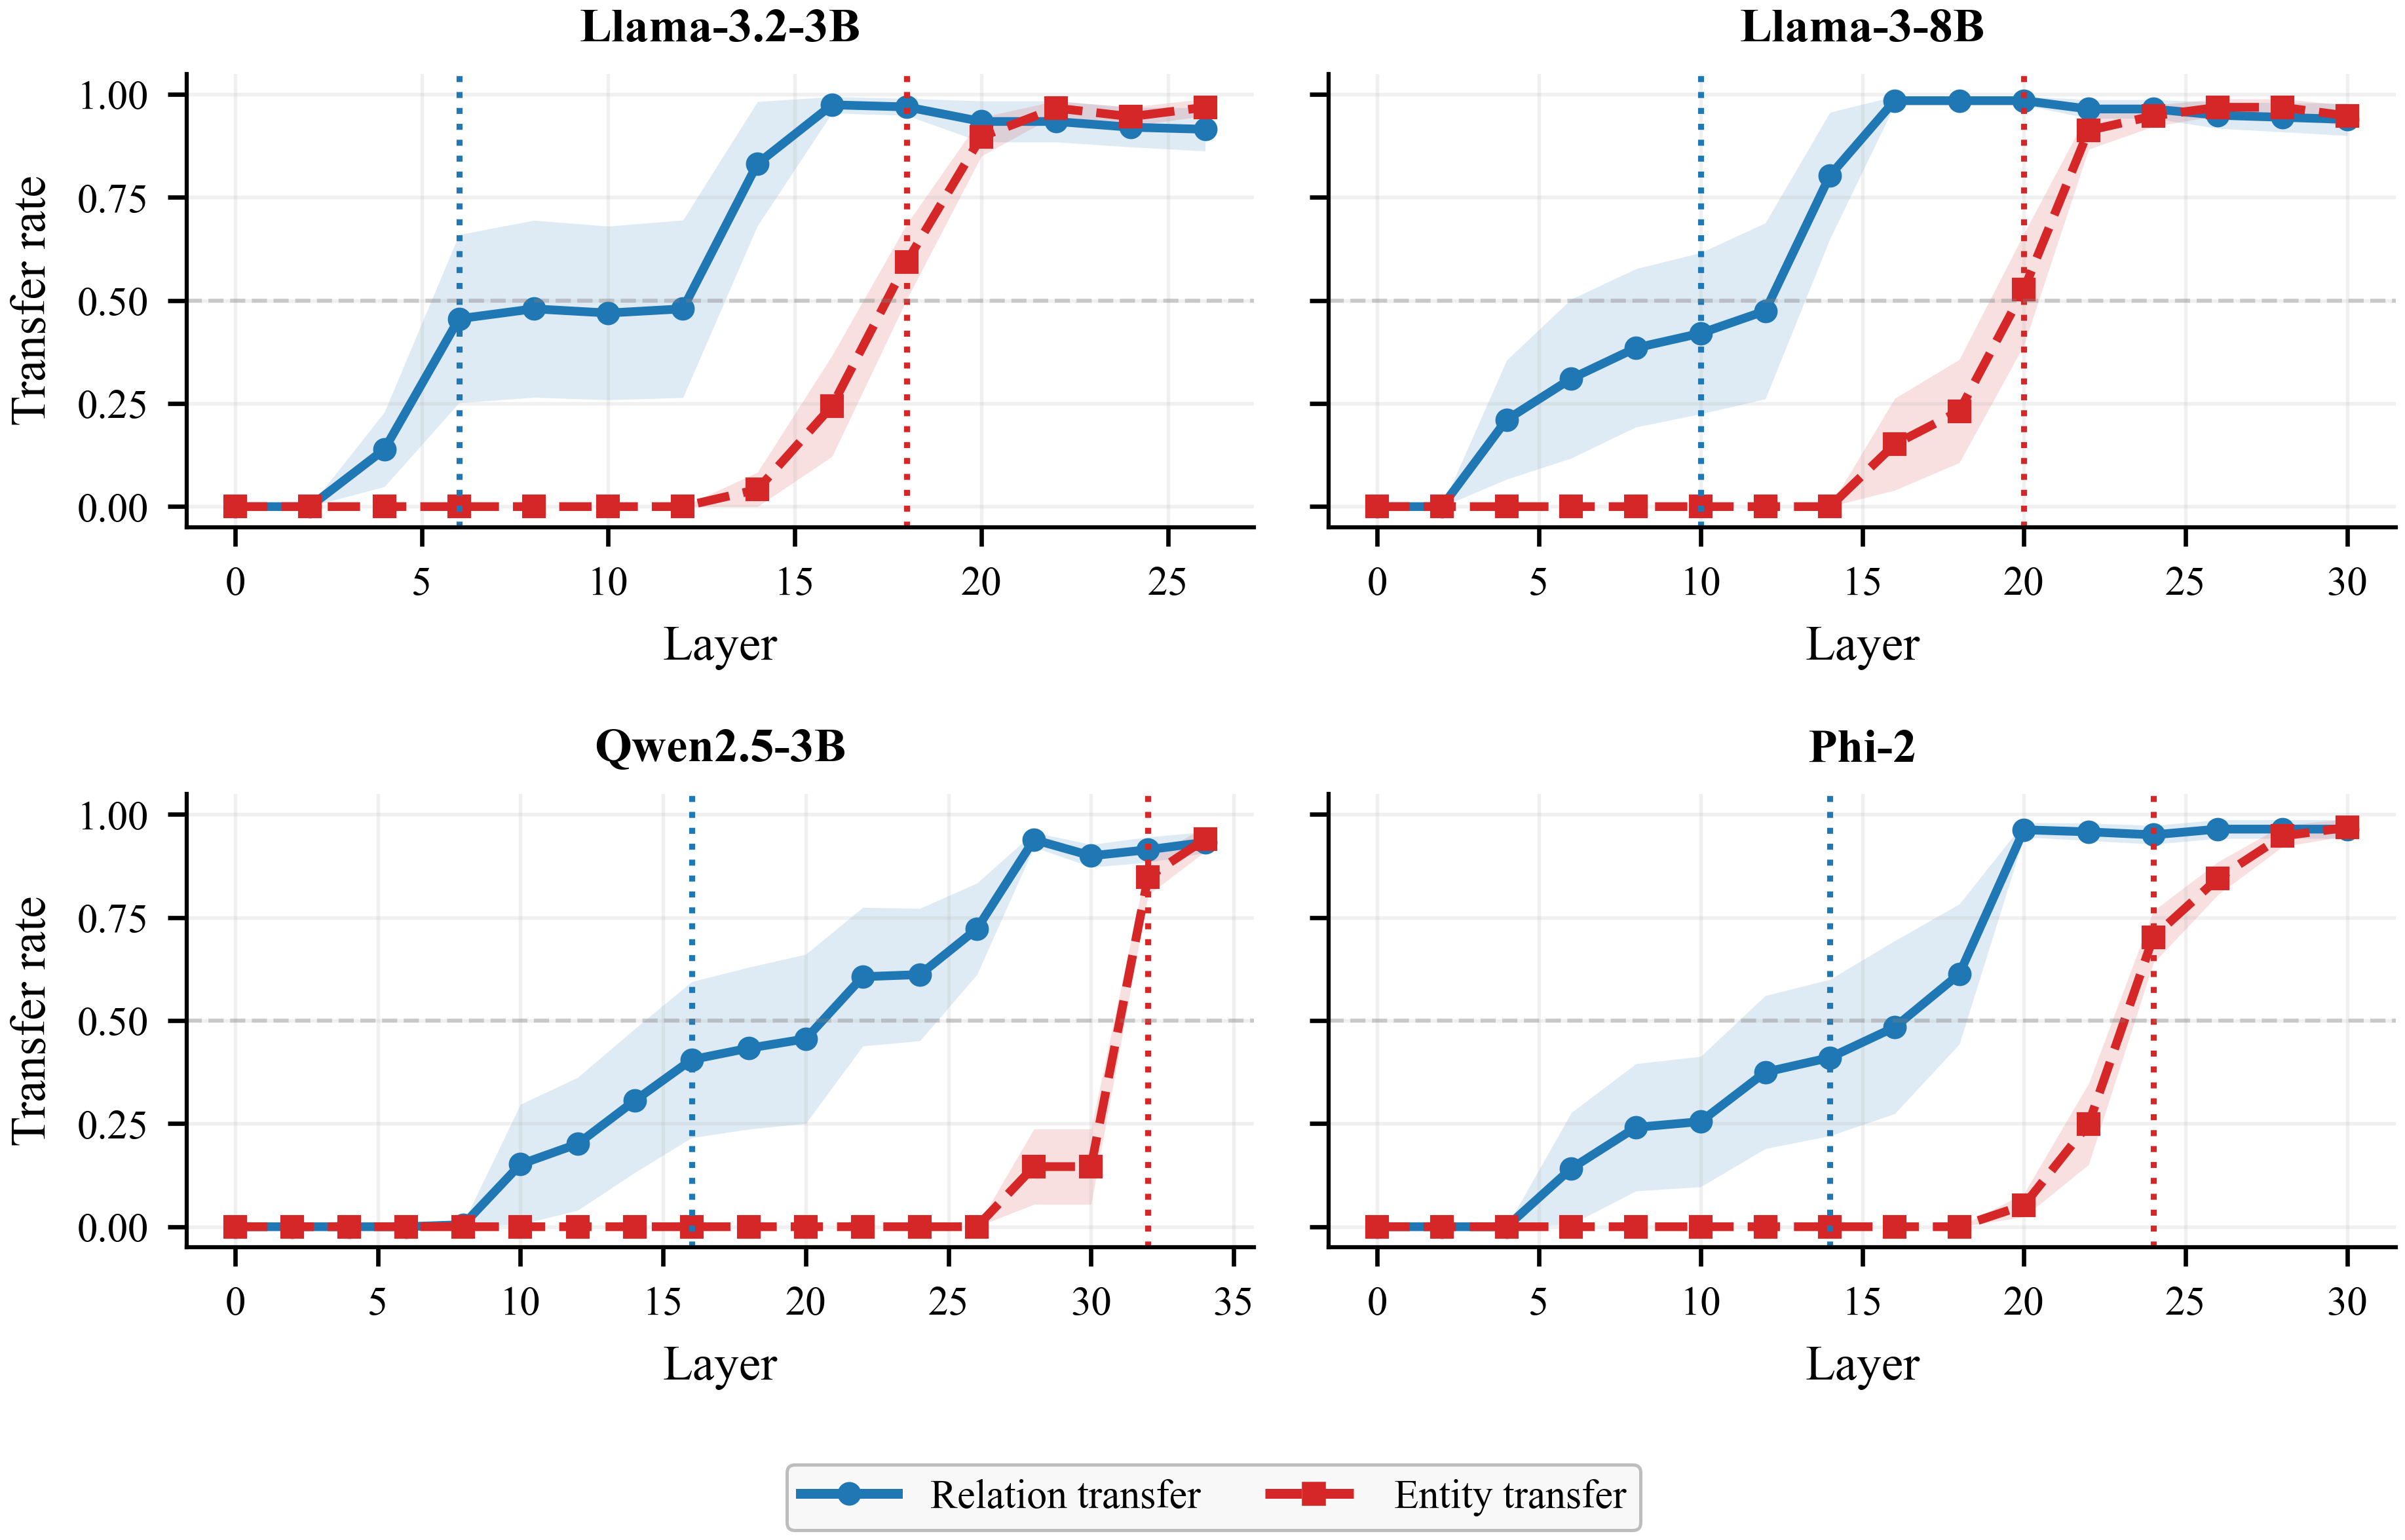
\includegraphics[width=0.80\linewidth]{figures/fig2_transfer_curves.png}
\caption{Relation transfer (blue) rises before entity transfer (red) in every model. Entity transfer is near zero for many consecutive layers while relation transfer already exceeds 0.4--0.8.}
\end{figure}

\section*{When they fight, relation wins early; entity wins late}

In the next experiment I changed \emph{both} the relation and the entity at the donor, forcing the two signals into direct competition. Outputs get classified as relation-wins, entity-wins, original-retained, or mixed. Relation-wins dominate the middle layers in every model; entity-wins take over in the late layers; the crossover tracks the entity onset from the previous experiment to within $\leq 2$ tested layers. Controls are clean: noise-patch yields $\leq 0.008$ structured wins, self-patch preserves the original output at $\geq 99.2\%$, and unrelated-donor patches produce \emph{high} late entity-like overwrite but \emph{near-zero} relation-wins ($\leq 0.030$) --- so mid-layer relation dominance is a real structured effect, not a generic patching artifact.

\section*{The key control: entity is already \emph{there}, just not \emph{used} yet}

The most obvious alternative explanation for everything above is: ``maybe entity information is just absent in early layers, and there's nothing interesting going on.'' To test this I patched at the \emph{entity-token} position instead of the final-token position. If the entity is genuinely missing early, entity-token patching should fail early too. If the entity is sitting there but hasn't been routed to the final token yet, it should work early at the entity-token position and only later at the final-token position.

\begin{center}\small
\begin{tabular}{lcc}
\toprule
Where the patch happens & Early layers & Late layers \\
\midrule
At the entity-token position & 90--100\% & 2--4\% \\
At the final-token position  & $\approx$2.4\% & 88--97\% \\
\bottomrule
\end{tabular}
\end{center}

A clean double dissociation. Entity information is \emph{strongly} usable from the earliest layers --- but only at the entity-token position. The final token is not yet causally controlled by entity-specific information; that information appears to reach the final position later via routing. The switch layer matches the entity onset from the first two experiments in every model. \emph{The information is available early, but not yet committed to generation.} I call this pattern \textbf{deferred entity commitment} which is delayed routing, not delayed knowledge.

\begin{figure}[h]
\centering
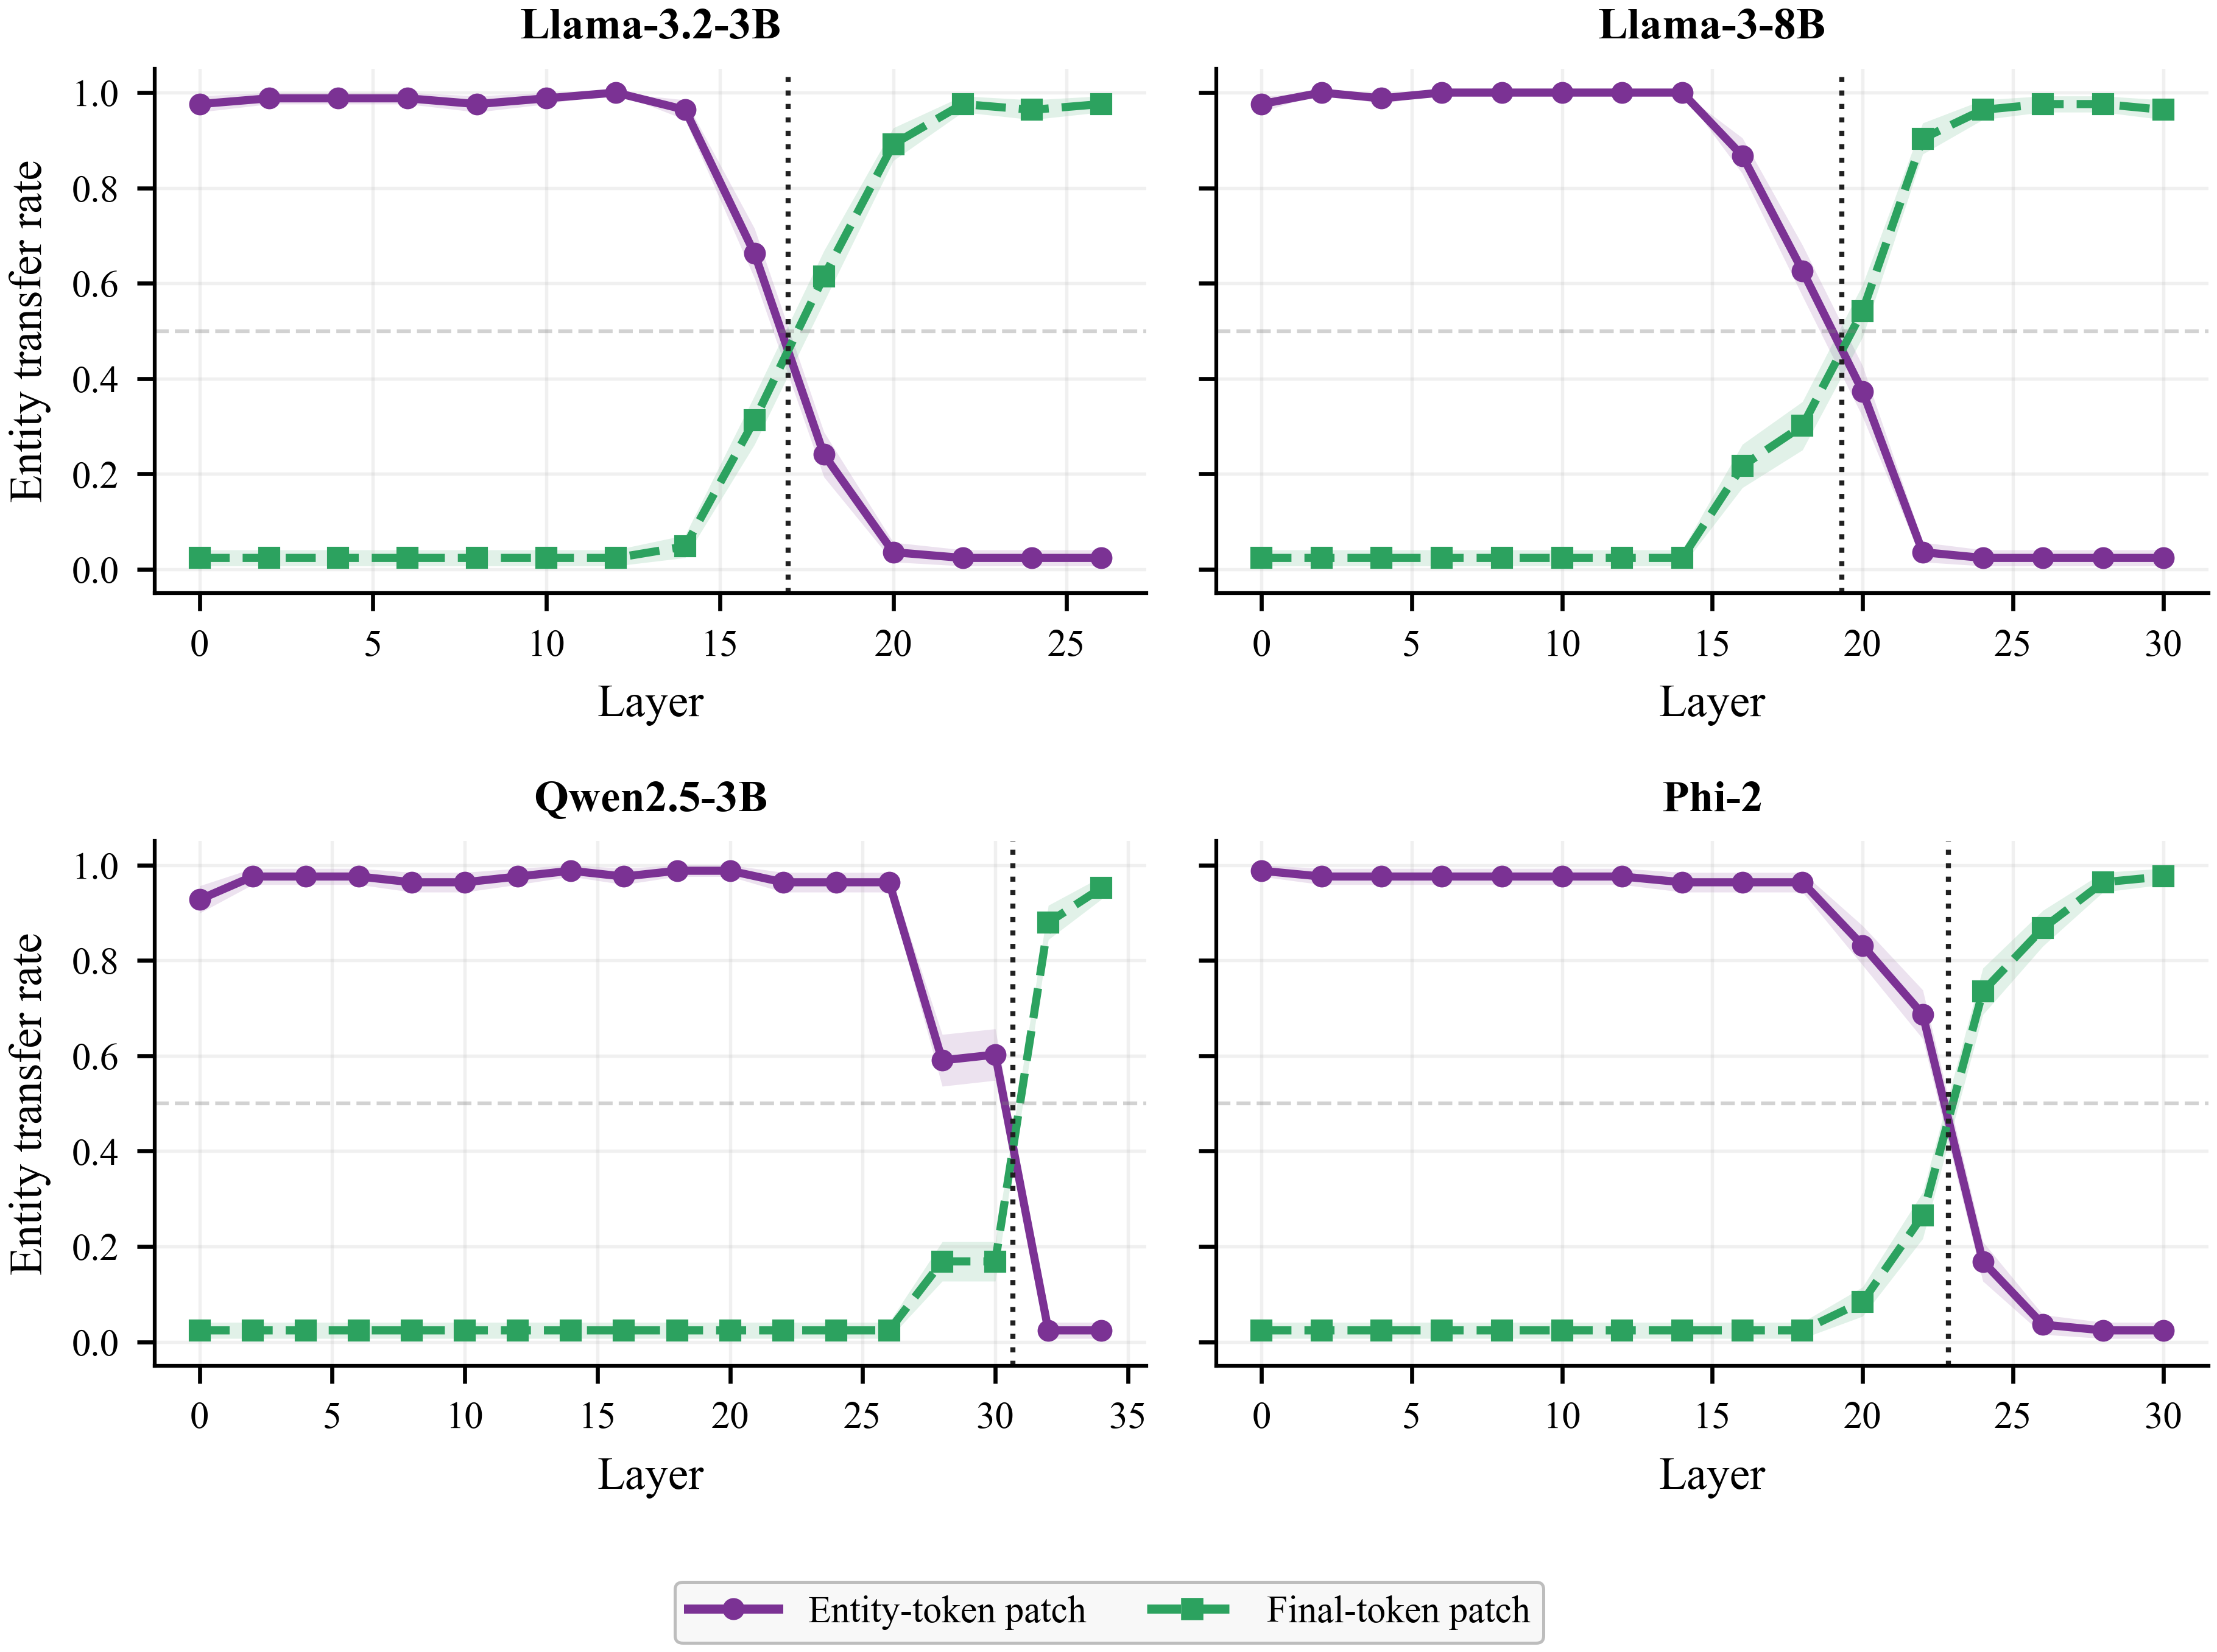
\includegraphics[width=0.80\linewidth]{figures/fig4_subject_vs_last_patching.png}
\caption{Entity-token patching (purple) succeeds at 90--100\% in early layers while final-token patching (green) is near zero. The pattern reverses late. Entity information exists early but only reaches the final token after being routed there.}
\end{figure}

\section*{Steering gives the same picture by an independent method}

As a sanity check using a different intervention, I built relation steering directions (mean-difference across same-entity/different-relation prompts) and entity steering directions (same-relation/different-entity), and applied them at mid- and late-layer zones. Relation directions steer effectively in middle layers; entity directions are substantially weaker mid-layer and strongest late. Random-direction baselines stay $\leq 0.015$. Same temporal asymmetry, completely different intervention.

\section*{What I think is going on}

Four complementary causal diagnostics converge on the same transition layers in every model, supporting a four-stage picture of recall:

\begin{enumerate}\setlength\itemsep{0em}\setlength{\parskip}{0pt}
  \item \textbf{Early:} entity is locally available at the entity-token position.
  \item \textbf{Middle:} relation information becomes generation-controlling at the final token.
  \item \textbf{Late:} entity information becomes generation-controlling at the final token (committed).
  \item \textbf{Latest:} the final-token state becomes more broadly overwrite-sensitive.
\end{enumerate}

The conceptual upshot is that two things routinely conflated in interp work which is \emph{representing} information and \emph{using} information to control generation come apart cleanly here. Entity-token patching succeeds from the earliest layers; final-token patching only succeeds much later. The entity is causally accessible at its own token from the start, but not causally controlling the generation position until late. Both are true at once.

\section*{Why this matters}

If relation and entity become generation-controlling at different depths, then (a) layer-targeted interventions like model editing or activation steering may hit relation-type and answer-identity computation very differently depending on \emph{where} they're applied; (b) decodability-based monitoring methods need to distinguish information availability from causal commitment, or they'll mis-classify what the model ``knows''; (c) similar staging may matter for chain-of-thought and multi-hop reasoning, where multiple relation-entity bindings have to be sequenced.

\section*{What I'd do next}

Three obvious extensions. (a) Localise the routing mechanism with attention-pattern analysis and head-level patching to know which heads carry the entity forward? (b) Scaling: does the relation--entity gap shrink, grow, or stay invariant with model size and instruction-tuning? (c) Extend to multi-hop and chain-of-thought prompts where multiple bindings have to be staged in sequence. The patching/steering infrastructure in the repo is a starting point for these follow-ups.

\section*{Limitations}

Controlled fill-in-the-blank families and greedy first-answer generation, so naturalistic QA and free-form reasoning aren't tested. Absolute layer numbers shouldn't be read as universal across the 3B--8B range. This is a robust timing asymmetry, not a complete circuit as the routing mechanism that moves entity information from the entity-token position to the final-token position isn't localised here.

\end{document}